\section{Tái hiện thuật toán}
\label{sec:reimplementation}

Toàn bộ mã nguồn của reimplementation được công bố tại:
\begin{center}
    \url{https://github.com/ptrnghieu/image-denoising-using-dfb-reimplement-and-improvements}
\end{center}

Phần này trình bày chi tiết quá trình reimplementation thuật toán khử nhiễu sử dụng DFB của Rosiles và Smith \cite{rosiles2000}. Do tính phức tạp của critically-sampled DFB với quincunx decimation, chúng tôi áp dụng một undecimated DFB trong miền tần số — một lựa chọn được biện giải kỹ ở mục~\ref{subsec:undecimated}. Các phần còn lại mô tả từng thành phần của pipeline.

% -----------------------------------------------------------------------
\subsection{Critically-sampled DFB vs.\ Undecimated DFB}
\label{subsec:undecimated}

\textbf{Critically-sampled DFB (paper gốc).}
Trong paper của Rosiles và Smith \cite{rosiles2000}, DFB được cài đặt theo đúng công trình gốc của Bamberger và Smith \cite{bamberger1992}: tại mỗi tầng của binary tree, tín hiệu được lọc bởi diamond filter rồi được downsampled bằng quincunx matrix. Sau $l = 3$ tầng, thu được 8 directional subband, mỗi subband chỉ còn $1/8$ tổng số pixel của ảnh gốc. Tính critically-sampled đảm bảo không có redundancy, và quincunx downsampling tạo ra các hệ số có phân bố sparse: tại các vị trí có cạnh theo đúng hướng của subband, hệ số lớn; còn lại gần bằng không.

\textbf{Undecimated DFB (cài đặt trong báo cáo này).}
Việc cài đặt critically-sampled DFB đòi hỏi xử lý quincunx lattice (lưới chéo không chữ nhật), polyphase decomposition, và thiết kế diamond filter compact — một quá trình phức tạp đáng kể về mặt kỹ thuật. Thay vào đó, chúng tôi sử dụng undecimated DFB: các directional filter được thiết kế trực tiếp trong miền tần số và áp dụng trên toàn bộ ảnh mà không có bất kỳ downsampling nào. Mỗi subband có cùng kích thước với ảnh đầu vào, tạo nên một overcomplete representation.

Cụ thể, mặt phẳng tần số 2D được phân chia thành $N$ vùng hình nêm bằng các cửa sổ raised-cosine trơn $H_k(\omega_1, \omega_2)$, $k = 0, \ldots, N-1$, thỏa mãn điều kiện partition of unity:

\begin{equation}
    \sum_{k=0}^{N-1} H_k(\omega_1, \omega_2) = 1
    \quad \forall\, (\omega_1, \omega_2)
    \label{eq:partition_unity}
\end{equation}

Điều kiện \eqref{eq:partition_unity} đảm bảo perfect reconstruction: khi không có biến đổi nào trên các subband, tổng của chúng cho lại ảnh gốc. Mỗi filter $H_k$ bao gồm cả wedge tại góc $\theta_k$ và wedge đối xứng $\theta_k + \pi$ do tính conjugate symmetry của phổ DFT của ảnh thực.

Undecimated DFB có một số ưu điểm quan trọng so với critically-sampled DFB trong bối cảnh denoising:
\begin{itemize}
    \item \textbf{Shift-invariance:} Không có downsampling nên kết quả không phụ thuộc vào vị trí của ảnh trong lưới lấy mẫu, tránh các Gibbs artifact điển hình của decimated filter bank.
    \item \textbf{Không có aliasing:} Critically-sampled DFB có thể xuất hiện aliasing do quincunx downsampling; undecimated DFB không có vấn đề này.
    \item \textbf{Dễ cài đặt và kiểm chứng:} Toàn bộ quá trình thực hiện qua FFT 2D, cho phép kiểm tra trực tiếp trong miền tần số.
\end{itemize}

% -----------------------------------------------------------------------
\subsection{Thiết kế directional filter}

Góc tại mỗi điểm $(\omega_1, \omega_2)$ trong mặt phẳng tần số được xác định bởi:

\begin{equation}
    \theta(\omega_1, \omega_2) = \arctan\!\left(\frac{\omega_1}{\omega_2}\right) \in [-\pi, \pi)
\end{equation}

Đối với $N$ directional subband, mỗi band $k$ có góc trung tâm:

\begin{equation}
    \theta_k = k \cdot \frac{\pi}{N} - \frac{\pi}{2} + \frac{\pi}{2N}, \quad k = 0, \ldots, N-1
\end{equation}

Filter của band $k$ được xây dựng từ cửa sổ raised-cosine:

\begin{equation}
    W(\theta;\, \theta_c,\, \Delta) =
    \begin{cases}
        1 & \text{nếu } |\theta - \theta_c| \leq \Delta/2 \\[4pt]
        \dfrac{1}{2}\!\left(1 + \cos\!\dfrac{\pi(|\theta - \theta_c| - \Delta/2)}{\Delta/2}\right)
          & \text{nếu } \Delta/2 < |\theta - \theta_c| \leq \Delta \\[4pt]
        0 & \text{ngược lại}
    \end{cases}
\end{equation}

với $\Delta = \pi/N$ là half-bandwidth của mỗi band. Filter $H_k$ trong miền tần số là:

\begin{equation}
    \tilde{H}_k(\omega_1, \omega_2)
    = W\!\bigl(\theta(\omega_1,\omega_2);\, \theta_k,\, 1.2\Delta\bigr)
    + W\!\bigl(\theta(\omega_1,\omega_2);\, \theta_k + \pi,\, 1.2\Delta\bigr)
\end{equation}

Hệ số $1.2$ tạo overlap nhỏ giữa các band liền kề để partition sau khi chuẩn hóa không có discontinuity. Sau đó chuẩn hóa để thỏa mãn \eqref{eq:partition_unity}:

\begin{equation}
    H_k(\omega_1, \omega_2)
    = \frac{\tilde{H}_k(\omega_1, \omega_2)}{\displaystyle\sum_{j=0}^{N-1} \tilde{H}_j(\omega_1, \omega_2)}
\end{equation}

\begin{figure}[H]
    \centering
    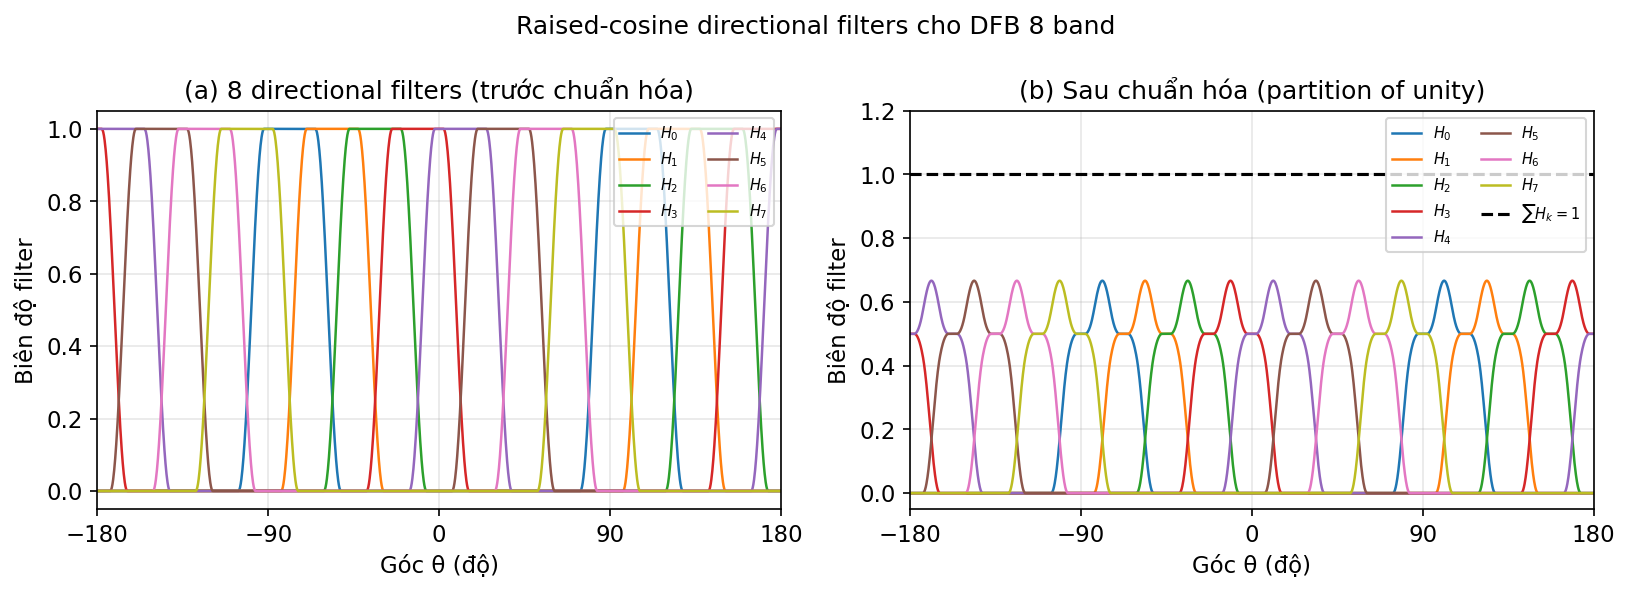
\includegraphics[width=\textwidth]{figures/raised_cosine_partition.png}
    \caption{Hình dạng các filter trong miền tần số góc. \textit{Trái:} ba filter $\tilde{H}_k$ trước khi chuẩn hóa, có overlap nhỏ tại ranh giới. \textit{Phải:} sau khi chuẩn hóa, tổng các filter bằng 1 tại mọi tần số (partition of unity).}
    \label{fig:raised_cosine}
\end{figure}

% -----------------------------------------------------------------------
\subsection{Vấn đề sparse representation và kỹ thuật LP/HP split}
\label{subsec:lphp}

\textbf{Vấn đề với full-spectrum wedge filter.}
Một điểm then chốt cần lưu ý là các full-spectrum wedge filter $H_k$ phủ toàn bộ dải tần số, từ DC đến Nyquist, theo hướng $\theta_k$. Do đó, mỗi directional subband $y_k = \mathcal{F}^{-1}\{X \cdot H_k\}$ chứa cả thành phần tần số thấp (smooth background) lẫn tần số cao (edges, texture). Kết quả là các subband này \emph{không sparse}: ngay cả ở các vùng phẳng (không có edge), hệ số vẫn có giá trị đáng kể do năng lượng DC.

Trong khi đó, các phương pháp thresholding như SURE và BayesShrink được thiết kế dưới giả định rằng signal có biểu diễn sparse trong miền transform: hầu hết các hệ số gần bằng không và chỉ một số ít hệ số lớn tại vị trí có signal. Khi điều này không thỏa mãn, thresholding với threshold lớn sẽ xóa cả signal, còn threshold nhỏ không loại bỏ được noise --- dẫn đến hiệu quả denoising kém.

\textbf{Kỹ thuật LP/HP split.}
Để khắc phục, chúng tôi áp dụng kỹ thuật tách ảnh thành thành phần lowpass (LP) và highpass (HP) trước khi áp dụng DFB. Cụ thể:

\begin{equation}
    \text{LP} = G_\sigma * y, \qquad \text{HP} = y - \text{LP}
    \label{eq:lphp}
\end{equation}

trong đó $G_\sigma$ là Gaussian kernel với $\sigma = 2.0$ pixel. Thành phần LP chứa hầu hết năng lượng tần số thấp của ảnh và gần như noise-free (do Gaussian blur trung bình hóa noise hiệu quả ở tần số thấp). Thành phần HP chứa các cạnh, texture và noise --- và quan trọng hơn, \emph{HP là sparse}: tại các vùng phẳng, HP $\approx 0$; chỉ tại các cạnh và texture mới có giá trị lớn.

\begin{figure}[H]
    \centering
    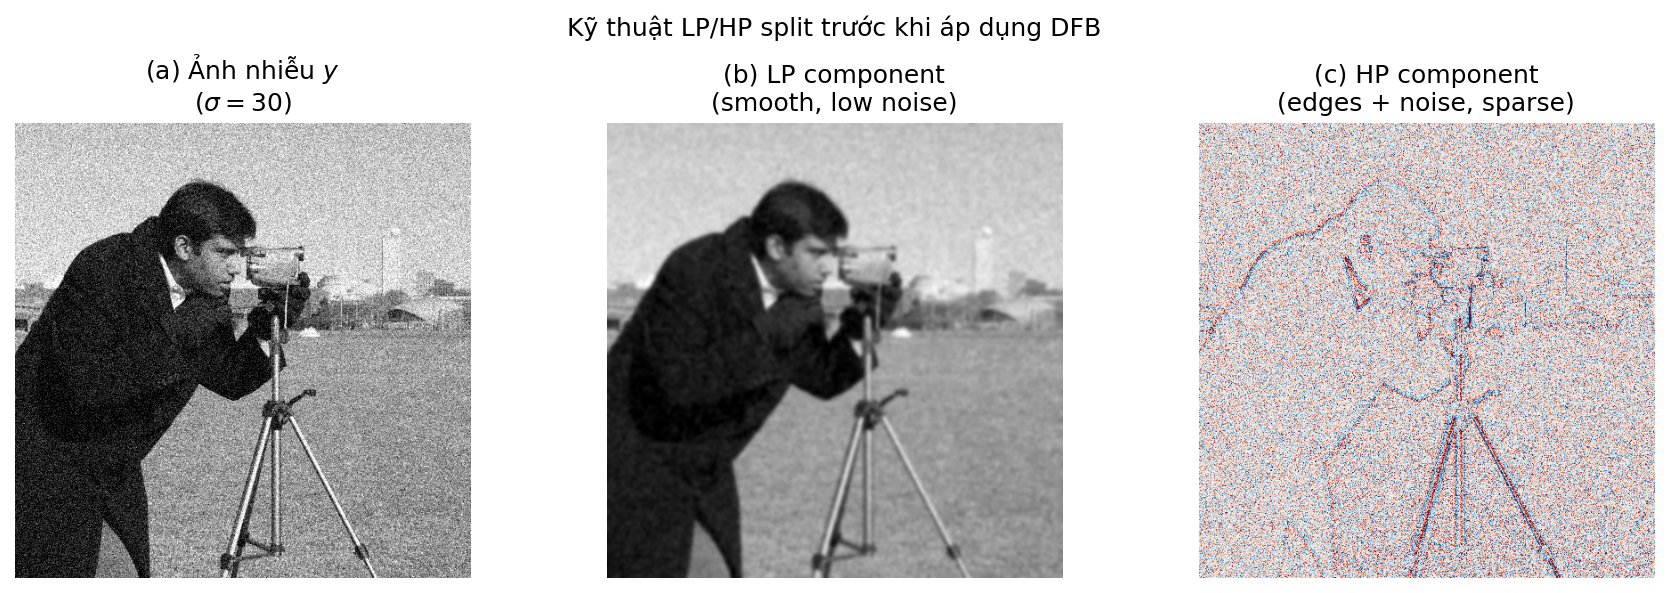
\includegraphics[width=\textwidth]{figures/lp_hp_split.png}
    \caption{Minh họa kỹ thuật LP/HP split trên ảnh Camera nhiễu ($\sigma = 20$). \textit{Trái:} ảnh nhiễu $y$. \textit{Giữa:} thành phần lowpass LP $= G_2 * y$ (mịn, gần như noise-free). \textit{Phải:} thành phần highpass HP $= y - \text{LP}$ (sparse, tập trung tại cạnh và texture).}
    \label{fig:lphp_split}
\end{figure}

\begin{figure}[H]
    \centering
    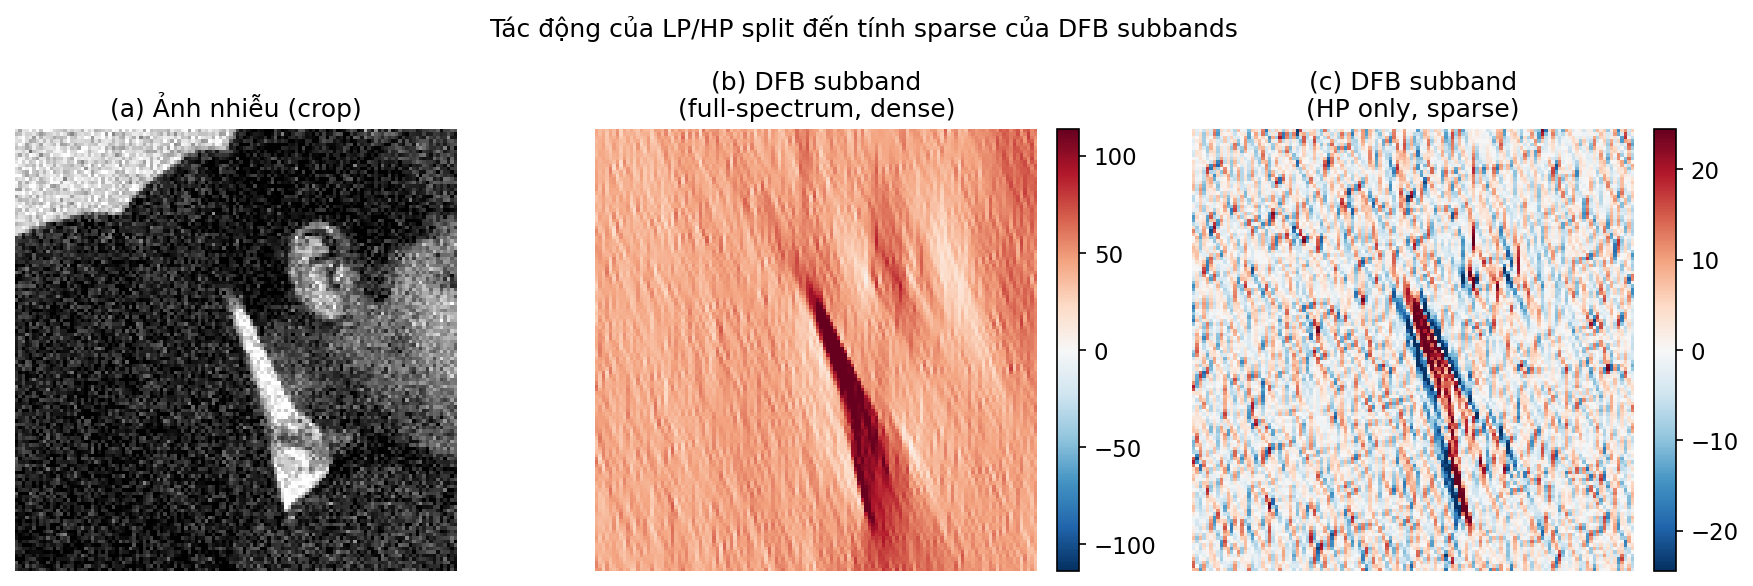
\includegraphics[width=\textwidth]{figures/dense_vs_sparse.png}
    \caption{So sánh directional subband số 0 của DFB 8 band. \textit{Trái:} subband của ảnh nhiễu đầy đủ (dense --- không sparse). \textit{Phải:} subband của thành phần HP (sparse --- hầu hết hệ số $\approx 0$, chỉ có cạnh theo hướng tương ứng có giá trị lớn). Sparsity là điều kiện cần cho thresholding hiệu quả.}
    \label{fig:dense_vs_sparse}
\end{figure}

DFB sau đó chỉ được áp dụng lên thành phần HP. Các directional subband của HP có phân bố sparse --- điều kiện cần thiết cho thresholding hoạt động hiệu quả. Ảnh được tái tạo bằng:

\begin{equation}
    \hat{x} = \text{LP} + \sum_{k=0}^{N-1} \eta_{t_k}(y_k^{\text{HP}})
    \label{eq:reconstruction}
\end{equation}

trong đó $y_k^{\text{HP}} = \mathcal{F}^{-1}\{X^{\text{HP}} \cdot H_k\}$ là directional subband thứ $k$ của HP, và $\eta_{t_k}$ là soft thresholding với ngưỡng $t_k$.

% -----------------------------------------------------------------------
\subsection{Ước lượng noise sigma}

Để ước lượng $\sigma$ từ ảnh nhiễu mà không cần biết giá trị thực, chúng tôi sử dụng MAD estimator áp dụng trên subband diagonal của wavelet bậc nhất (Haar), theo Donoho và Johnstone \cite{donoho1995}:

\begin{equation}
    \hat{\sigma} = \frac{\operatorname{median}(|d|)}{0.6745}
    \label{eq:sigma_hat}
\end{equation}

trong đó $d$ là tập hệ số của detail subband diagonal ở bậc phân giải mịn nhất (thu được qua một bước DWT với Haar wavelet). Subband diagonal được chọn vì nó chứa ít signal nhất và noise chiếm ưu thế, giúp ước lượng $\sigma$ ít bị bias bởi tín hiệu.

\textbf{Per-subband noise sigma.}
Khi DFB được áp dụng lên thành phần HP, mỗi directional subband nhận một phần noise từ HP. Với partition-of-unity filters ($\sum_k H_k = 1$), năng lượng noise phân bổ đều qua các subband. Variance của noise trong subband thứ $k$ là:

\begin{equation}
    \sigma_k^2 = \sigma_{\text{HP}}^2 \cdot \frac{1}{MN} \sum_{\omega_1, \omega_2} H_k^2(\omega_1, \omega_2) \approx \frac{\sigma_{\text{HP}}^2}{N}
\end{equation}

Do đó:

\begin{equation}
    \sigma_k = \frac{\sigma_{\text{HP}}}{\sqrt{N}}
    \label{eq:sigma_k}
\end{equation}

với $\sigma_{\text{HP}} \approx \hat{\sigma}$ (Gaussian LP filter với $\sigma = 2$ loại bỏ ít noise nên $\sigma_{\text{HP}} \approx \sigma$). Giá trị $\sigma_k$ được dùng làm đầu vào cho các threshold estimator ở bước tiếp theo.

% -----------------------------------------------------------------------
\subsection{Threshold selection}

Với mỗi directional subband $y_k^{\text{HP}}$ của HP, threshold $t_k$ được ước lượng theo các phương pháp sau.

\textbf{SURE.}
Từ công thức \eqref{eq:sure}, để áp dụng đúng, các hệ số cần được chuẩn hóa về noise variance bằng 1. Đặt $z_i = y_i / \sigma_k$, ta minimize:

\begin{equation}
    \tilde{t}_k^* = \arg\min_{\tilde{t} \geq 0}
    \left[
        n - 2 \cdot \#\{|z_i| \leq \tilde{t}\}
        + \sum_i \min(z_i^2,\, \tilde{t}^2)
    \right]
\end{equation}

Threshold trong đơn vị gốc là $t_k = \tilde{t}_k^* \cdot \sigma_k$. Việc chuẩn hóa là bắt buộc: nếu bỏ qua, hàm SURE không có nghĩa thống kê và luôn cho $t_k \approx 0$ (không threshold), như chúng tôi đã xác nhận qua thực nghiệm.

\textbf{GCV.}
Tương tự, trong miền chuẩn hóa $z_i = y_i/\sigma_k$:

\begin{equation}
    \tilde{t}_k^* = \arg\min_{\tilde{t} \geq 0}
    \frac{\displaystyle\sum_i \min(z_i^2,\, \tilde{t}^2)}
    {\!\left(\dfrac{\#\{|z_i| \leq \tilde{t}\}}{n}\right)^{\!2}}
\end{equation}

\textbf{MAD + universal threshold.}
Sigma được ước lượng từ subband bằng MAD và áp dụng universal threshold:

\begin{equation}
    t_k = \sigma_k \sqrt{2 \log n}
\end{equation}

trong đó $n$ là số phần tử của subband.

% -----------------------------------------------------------------------
\subsection{Tổng kết pipeline và pseudocode}

Hình~\ref{fig:pipeline} mô tả toàn bộ pipeline của thuật toán reimplementation. Pseudocode được trình bày trong Algorithm~\ref{alg:dfb_denoise}.

\begin{figure}[H]
    \centering
    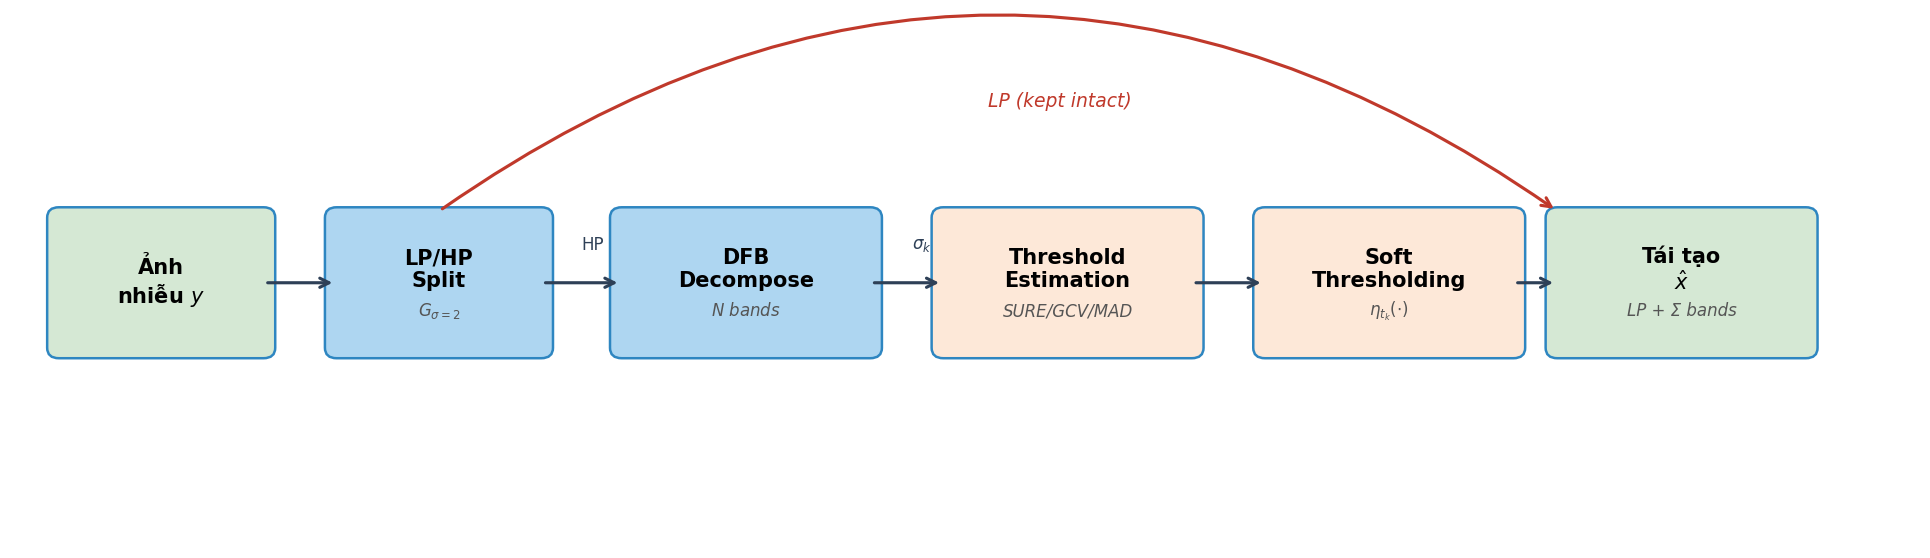
\includegraphics[width=0.85\textwidth]{figures/pipeline.png}
    \caption{Pipeline của thuật toán DFB denoising (reimplementation).
             LP được giữ nguyên; DFB và thresholding chỉ áp dụng lên HP.}
    \label{fig:pipeline}
\end{figure}

\begin{algorithm}[H]
\caption{DFB Image Denoising}
\label{alg:dfb_denoise}
\begin{algorithmic}[1]
\Require Ảnh nhiễu $y$, số band $N$, phương pháp threshold $m$, sigma nhiễu $\sigma$ (tùy chọn)
\Ensure Ảnh khử nhiễu $\hat{x}$

\State Ước lượng $\hat{\sigma}$ từ wavelet diagonal subband theo \eqref{eq:sigma_hat} (nếu $\sigma$ chưa cho)
\State Tính $\text{LP} \gets G_{\sigma=2} * y$ và $\text{HP} \gets y - \text{LP}$
\State Tính $X^{\text{HP}} \gets \mathcal{F}\{\text{HP}\}$ \Comment{2D DFT của HP}
\State Xây dựng $N$ directional filter $H_0, \ldots, H_{N-1}$ (partition of unity)
\State Tính $\sigma_k \gets \hat{\sigma} / \sqrt{N}$ \Comment{per-subband noise sigma}
\For{$k = 0$ \textbf{to} $N-1$}
    \State $y_k \gets \mathcal{F}^{-1}\{X^{\text{HP}} \cdot H_k\}$ \Comment{directional subband}
    \State Tính $t_k$ theo phương pháp $m$ (SURE / GCV / MAD) với $\sigma_k$
    \State $\hat{y}_k \gets \eta_{t_k}(y_k)$ \Comment{soft thresholding}
\EndFor
\State $\hat{x} \gets \text{LP} + \sum_{k=0}^{N-1} \hat{y}_k$
\Return $\hat{x}$
\end{algorithmic}
\end{algorithm}

Độ phức tạp tính toán của thuật toán là $O(MN \log MN)$ cho mỗi lần DFT/IDFT, và $O(n \log n)$ cho mỗi lần tính SURE/GCV trên $n = MN$ hệ số. Tổng thể: $O(N \cdot MN \log MN)$ với $N$ directional band.
